\chapter{ПРОВЕДЕНИЕ АНАЛИЗА НОВОСТНЫХ ДАННЫХ}
\label{chap:research}
\aftertitle

В этой главе рассматривается экспериментальная работа по проверке разработанного сервиса и анализу новостей с его помощью. Описаны проведенные эксперименты по анализу новостей.

В исследовании использовались исторические данные новостей, собранные за 2020 год.

\section{Анализ количества новостей}

В первую очередь был произведен анализ количества новостей в день за исследуемый промежуток времени. На рисунке \ref{img:news-count} представлен график количества новостей за день. Минимальное количество новостей в день 165, максимальное ~-- 2890, а среднее ~--- 1907.

\begin{figure}[h]
    \centering
    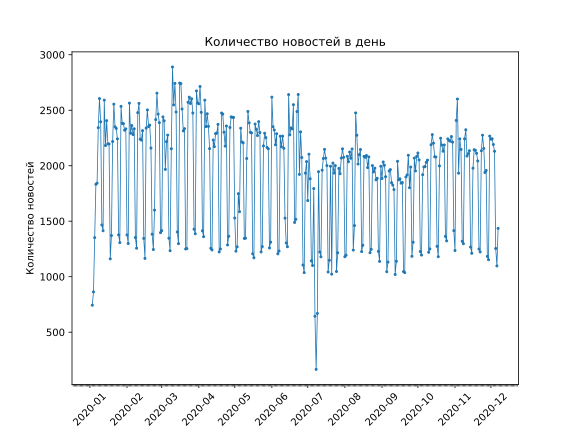
\includegraphics[width=\linewidth]{images/news-count.png}
    \caption{Количество новостей в день}
    \label{img:news-count}
\end{figure}

На этом графике мы можем видеть, что количество новостей в день оставалось примерно в одинаковом диапазоне на протяжении всего периода сбора данных. Отсутствие сильных выбросов (отличающихся в десятки раз) говорит о том, что, вероятно, ошибок в сборе данных допущено не было.

Интересным фактом является явный периодический характер изменения количества новостей по дням. Вероятнее всего, это недельные колебания количества новостей. В будние дни количество новостей больше, в то время как в выходные дни количество новостей существенно (в полтора-два раза) меньше.

\section{Исследование расстояния между новостями}

В рамках проведения анализа новостных данных, изучалась статистика попарного косинусного расстояния между векторным представлением новостей за день.

Косинусное расстояние двух векторов $a$ и $b$ ~-- это метрика схожести двух ненулевых векторов, определяемая как косинус угла между ними (\ref{eq:cosine-dist}).

\begin{equation}
    cos(\theta) = \frac{\vec{a} \cdot \vec{b}}{||\vec{a}|| \cdot ||{b}||}
    \label{eq:cosine-dist}
\end{equation}

Таким образом, эмбеддинги близких по смыслу новостей будут представлять собой два вектора с приблизительно одинаковым направлением, и их косинусное расстояние будет близко к единице. Наоборот, эмбеддинги противоположных по смыслу новостей будут представлять собой два вектора, направленные в противоположенные стороны, и их косинусное расстояние будет близко к минус единице. Таким образом, чем ближе косинусное расстояние к единице, тем более похожи новости.

Так как косинусное расстояние между векторным представлением соответствует семантической близости новостей друг другу, то статистика попарных расстояний может отражать характер распределения новостей по темам. Если за выбранный временной интервал много новостей на различные темы, то косинусное расстояние между ними будет близко к -1, и статистика попарных расстояния будут сдвинута в сторону меньших значений. Наоборот, если новости за выбранный временной интервал были на схожие темы, то косинусное расстояние будет близко к 1 , и статистика распределения попарных расстояний будет сдвинута в сторону больших значений.

На рисунке \ref{img:distances-distribution} показано сравнение распределения попарных косинусных расстояний за два дня. Распределение в области малых значений, т.е. новостей, которые не похожи друг на друга, совпадает. Различие наблюдается в области больших значений, т.е. новостей, которые похожи друг на друга. За один день наблюдается большее значение плотности распределения в области больших значений, чем за другой день, что говорит о том, что в этот день было больше новостей на близкие темы.

\begin{figure}[h]
    \centering
    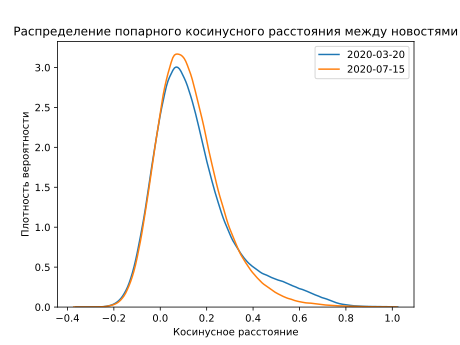
\includegraphics[width=\linewidth]{images/distances-distribution.png}
    \caption{Сравнение распределение косинусного расстояния между новостями за два дня}
    \label{img:distances-distribution}
\end{figure}

Так как построение распределения для всех дней не является наглядной визуализацией, то для изучения динамики изменения распределения попарных косинусных расстояний межу новостями, было решено построить графики отдельных квантилей: 50\% (медиана), 75\% и 90\%. График изменения распределения попарного косинусного расстояния по дням представлен на рисунке \ref{img:distances}.

\begin{figure}[h]
    \centering
    \includegraphics[width=\linewidth]{images/distances.png}
    \caption{Изменение распределения попарного косинусного расстояния по дням}
    \label{img:distances}
\end{figure}

На этом графике показаны значения трех перцентилей: 50\% (синий), 75\% (оранжевый) и 90\% (зеленый) в виде точек. Каждая точка показывает значение соответствующего квантиля распределения попарного косинусного расстояния между новостями за один день. На графике мы  можем отчетливо видеть колебания с периодом 7 дней, по всей видимости, связанные с недельными изменениями в  распределении тематик новостей.

Значения 50\% квантиля практически не изменяются во времени, не считая недельных колебаний. Это согласуется с рассмотренным ранее на рисунке \ref{img:distances-distribution} сравнением распределения попарных косинусных расстояний между новостями за два дня, на котором видно, что в области малых значений распределение практически совпадает. Медианное значение 50\%-квантиля составляет 0.12, что соответствует непохожим новостям. Таким образом, распределение непохожих новостей мало меняется во времени, что может говорить о том, что в новостях всегда (за исключением недельных колебаний) охватывается примерно одинаково широкий круг тем.

Поведение значения 75\% квантиля мало отличается от поведения значений 50\% квантиля, но в них наблюдается небольшое увеличение в определенные моменты времени.

Наибольший интерес представляет поведение 90\% квантиля. Среди этих значений недельные колебания не так выражены, но выражен значительный рост значений в определенный период времени. Это говорит о том, что в этот момент времени распределение попарных косинусных расстояний между новостями было смещено в область больших значений, т.е. было больше новостей на похожие темы. По времени этот момент совпадает с началом пандемии коронавируса, карантина и экономического кризиса. Вероятно, эти темы обсуждались более активно, чем другие, что вызвало появление большего количества новостей на сходные тематики и смещение распределения попарного косинусного расстояния между новостями.

Таким образом, исследование распределения попарного косинусного расстояния между новостями может служить инструментом для выявления периодов с активным обсуждением тех или иных тем. При этом, наибольший интерес представляют больше квантили, такие как 90\%-квантиль.

\section{Исследование кросс-корреляции с финансовым инструментом}

Реализованный в данной работе сервис позволяет оценивать корреляцию количества новостей по заданным темам с различными временными рядами. В качестве примера, была изучена кросс-корреляция количества новостей по различным темам с ценой финансового инструмента ~-- с курсом доллара по отношению  к рублю, чтобы изучить, как разработанный сервис может быть использован в исследованиях финансовых рынков.

Для этого использовалось API сервиса /api/v1/correlations. С помощью этого API определялось количество новостей по заданным темам за данные промежутки времени и рассчитывалась корреляция с курсом доллара. Количество новостей определялось за окно длительностью семь дней, которое сдвигалось с шагом шесть часов. Такое окно было выбрано, чтобы сгладить недельные колебания в количестве новостей. Таким образом, каждая точка на графике количества новостей представляет собой нормированное суммарное количество новостей за семь дней

Исторические данные о курсе доллара были взяты с веб-сайта "ФИНАМ" \cite{finam}. Данные представлены в формате CSV и состоят из пятнадцатиминутных интервалов. Каждый интервал характеризуется ценой открытия, ценой закрытия, минимальной ценой и максимальной ценой. Так как количество новостей рассчитывалось за окно длительностью семь дней, необходимо привести данные курса доллара к такому же виду. Для этого, в качестве значения курса доллара бралось медианное значение цены закрытия всех интервалов за окно длительностью семь дней. Аналогично, окно сдвигалось с шагом шесть часов. аким образом, каждая точка на графике курса доллара представляет собой медианную цену закрытия за семь дней.


Анализировалась корреляция абсолютного количества новостей с курсом доллара, корреляция относительного количества новостей с курсом доллара и корреляция абсолютного количества новостей с производной курса доллара.

\subsection{Корреляция количества новостей с курсом доллара}

Для исследования были выбраны следующие темы, которые могли бы быть актуальны на исследуемый период: экономика, политика, коронавирус, самоизоляция, курс доллара, фондовый рынок, нефть, кризис, акции.

Перед расчётом кросс-корреляции, значение количества новостей и стоимости доллара нормировались таким образом, чтобы попасть в диапазон $[-1; 1]$. Нормировка осуществлялась с помощью класса MinMaxScaler из библиотеки scikit-learn.

Графики корреляции количества новостей по теме <<нефть>> приведены на рисунках \ref{img:correlation-absolute-oil}. На верхних части графика показаны нормированные значения количества новостей (оранжевый) и курса доллара (синий). На нижней части графика показано значение корреляционной функции (синий).

\begin{figure}[h]
    \centering
    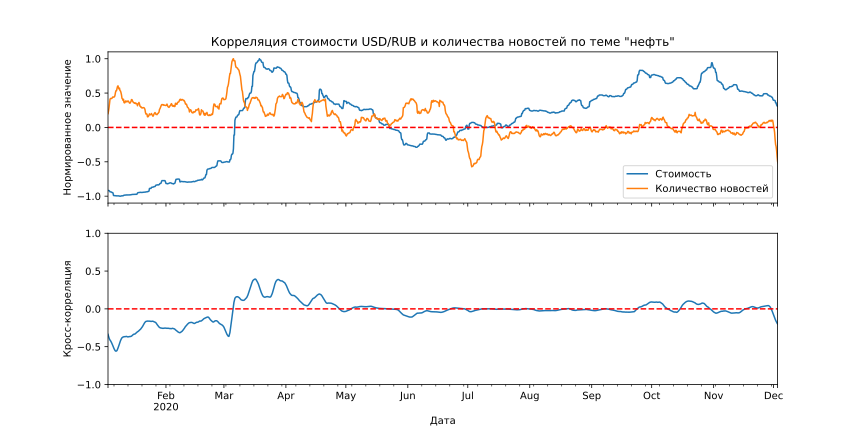
\includegraphics[width=\linewidth]{images/correlations/absolute/нефть.png}
    \caption{Корреляция количества новостей по теме <<нефть>> с курсом доллара}
    \label{img:correlation-absolute-oil}
\end{figure}

Графики корреляции количества новостей по теме <<коронавирус>> приведены на рисунках \ref{img:correlation-absolute-covid}. На верхних части графика показаны нормированные значения количества новостей (оранжевый) и курса доллара (синий). На нижней части графика показано значение корреляционной функции (синий).

\begin{figure}[h]
    \centering
    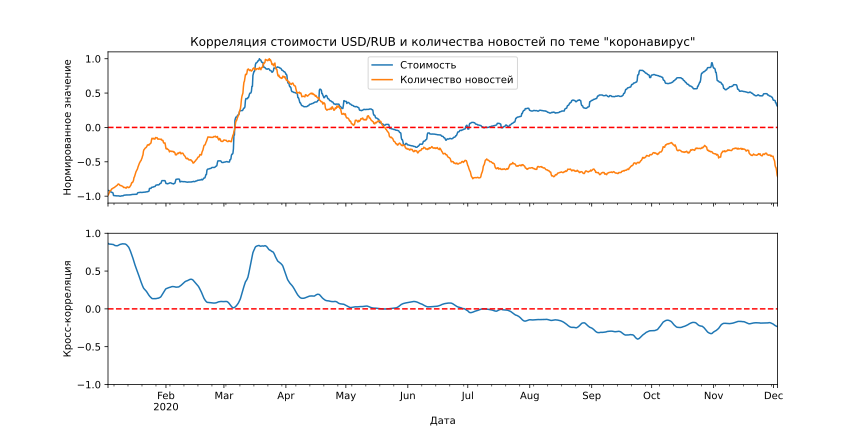
\includegraphics[width=\linewidth]{images/correlations/absolute/коронавирус.png}
    \caption{Корреляция количества новостей по теме <<коронавирус>> с курсом доллара}
    \label{img:correlation-absolute-covid}
\end{figure}

По данным графикам затруднительно сделать какие-либо выводы о влиянии изменения стоимости финансового инструмента на новости и наоборот. Мы видим слабую корреляцию курса доллара с количеством новостей по теме <<нефть>>. Мы видим сильную корреляцию в определенные моменты времени курса доллара с количеством новостей по теме <<коронавирус>> в момент резкого роста курса доллара.

\subsection{Корреляция относительного количества новостей с курсом доллара}

Рассмотрим аналогичные графики, но для относительного количества новостей. Количество новостей по той или иной теме было нормировано на общее количество новостей за день, чтобы не учитывать влияние количества новостей, а только относительную долю рассматриваемой теме в общем количестве новостей за заданный временной интервал.

Графики корреляции относительного количества новостей по теме <<нефть>> приведены на рисунке \ref{img:correlation-relative-oil}. На верхней части графика показаны нормированные значения количества новостей (оранжевый) и курса доллара (синий). На нижней половине графика показано значение корреляционной функции (синий).
\begin{figure}[h]
    \centering
    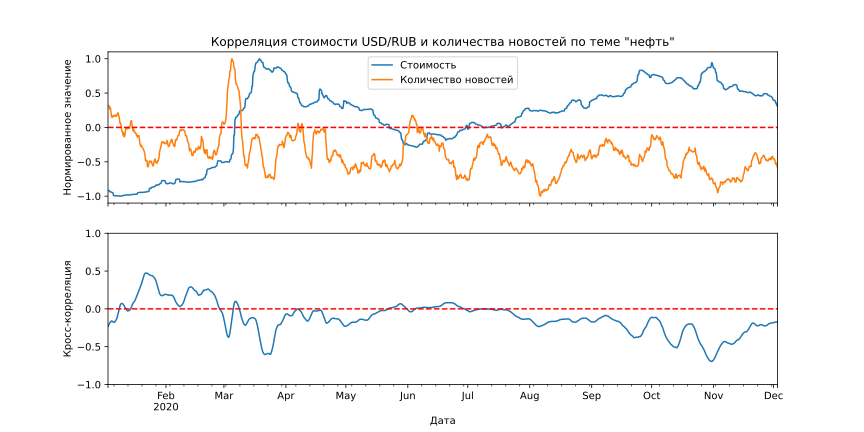
\includegraphics[width=\linewidth]{images/correlations/relative/нефть.png}
    \caption{Корреляция относительного количества новостей по теме <<нефть>> с курсом доллара}
    \label{img:correlation-relative-oil}
\end{figure}

Графики корреляции относительного количества новостей по теме <<коронавирус>> приведены на рисунке \ref{img:correlation-relative-covid}. На верхней части графика показаны нормированные значения количества новостей (оранжевый) и курса доллара (синий). На нижней половине графика показано значение корреляционной функции (синий).

\begin{figure}[h]
    \centering
    \includegraphics[width=\linewidth]{images/correlations/relative/коронавирус.png}
    \caption{Корреляция относительного количества новостей по теме <<коронавирус>> с курсом доллара}
    \label{img:correlation-relative-covid}
\end{figure}

По данным графикам затруднительно сделать какие-либо выводы о влияние изменения стоимости финансового инструмента на новости и наоборот.  Аналогично, мы видим слабую корреляцию курса доллара с количеством новостей по теме <<нефть>>. Мы видим сильную корреляцию в определенные моменты времени курса доллара с количеством новостей по теме <<коронавирус>>.

\subsection{Корреляция количества новостей с производной курса доллара}

Было выдвинуто предположение, что в новостях отражается не столько сам курс доллара, сколько его изменения. В периоды, когда курс доллара приблизительно стабилен, это не находит активного отражения в новостях. В периоды, когда происходят сильные колебания курса доллара, это находит активное отражение в новостях, как в специализирующихся на экономике изданиях, так и в общих средствах массовой информации.

Для того, чтобы проанализировать корреляцию количества новостей с изменениями курса доллара, курс доллара был численно дифференцирован. Для дифференцирования применялась центральная разностная схема (\ref{eq:derrivative}). Регулируя параметр шага можно влиять на сглаженность производной. Т.к. курс доллара имеет множество мелких колебаний, то для анализа только крупных изменений, шаг дифференцирования может быть увеличен.

\begin{equation}
    C'_i \approx \frac{C_{i+n} - C_{i-n}}{2n}
    \label{eq:derrivative}
\end{equation}
\noindent\begin{tabularx}{\linewidth}{lllX}
    где & $C_i$    &~--& стоимость в момент времени $i$, \\
        & $i$      &~--& момент времени, \\
        & $n$      &~--& шаг. \\
\end{tabularx}

Приведенные ниже результаты получены при значении шага $n = 4$ отсчёта.

На рисунке \ref{img:usd_derrivative} показан курс доллара (верхний график) и производная курса доллара (нижний график) за рассматриваемый период.

\begin{figure}[h]
    \centering
    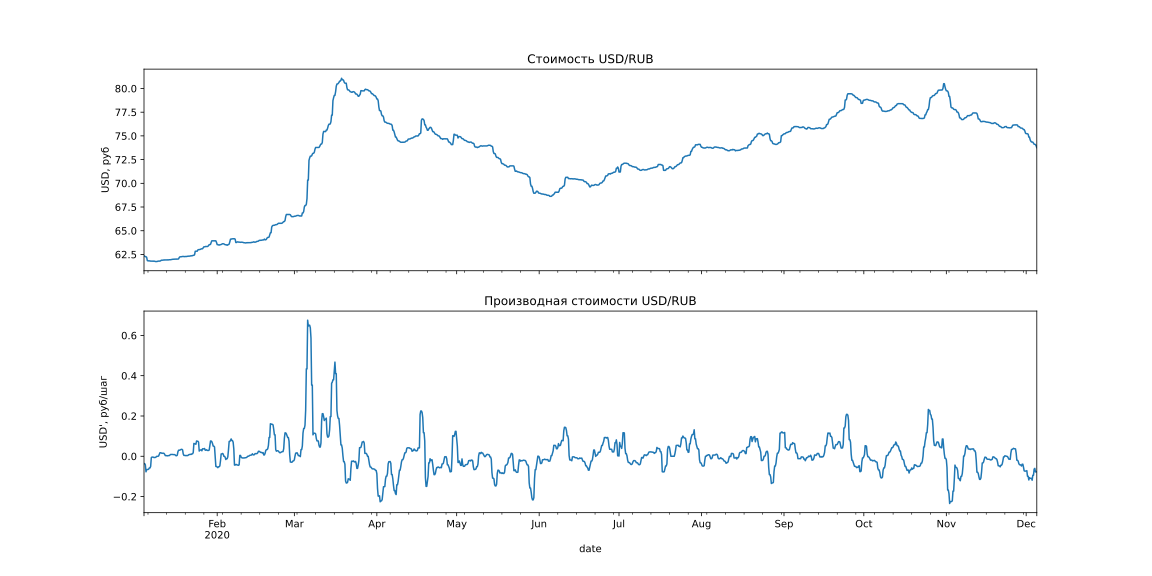
\includegraphics[width=\linewidth]{images/correlations/usd_derrivative.png}
    \caption{Производная курса доллара}
    \label{img:usd_derrivative}
\end{figure}

Для расчёта корреляции необходимо нормализовать данные. Но для производной курса доллара MinMaxScaler не подходит, потому что при его применении может произойти сдвиг нуля, а нуль имеет важное значение для производной курса, обозначая отсутствие изменений. Поэтому, был применен другой способ нормализации, который масштабирует размах функции в интервал $[-1; 1]$, но сохраняет положение нуля (\ref{eq:derr-normalize}). Данный способ определяет максимальный размах значения функции от нуля и масштабирует ее таким образом, чтобы максимальный размах составлял единицу.

\begin{equation}
    \begin{array}{l}
        k = max(max(C'), -min(C')), \\
        C'_{norm} = k \cdot C'
    \end{array}
    \label{eq:derr-normalize}
\end{equation}\noindent\begin{tabularx}{\linewidth}{lllX}
    где & $C'$         &~--& производная стоимости, \\
        & $C'_{norm}$  &~--& нормированная производная стоимости. \\
\end{tabularx}


Используя рассмотренный способ нормализации, была рассчитана корреляция между количеством новостей по определенным темам и производной курса доллара.

Графики корреляции относительного количества новостей по теме <<нефть>> приведены на рисунке \ref{img:correlation-derrivative-oil}. На верхней части графика показаны нормированные значения количества новостей (оранжевый) и производная курса доллара (синий). На нижней части графика показано значение корреляционной функции (синий).

\begin{figure}[h!]
    \centering
    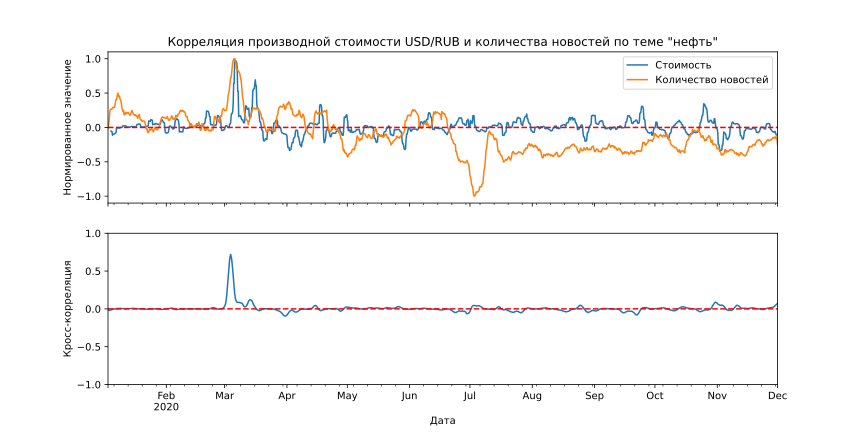
\includegraphics[width=\linewidth]{images/correlations/derivative/нефть.png}
    \caption{Корреляция количества новостей по теме <<нефть>> с производной курса доллара}
    \label{img:correlation-derrivative-oil}
\end{figure}

Графики корреляции относительного количества новостей по теме <<коронавирус>> приведены на рисунке \ref{img:correlation-derrivative-covid}. На верхней части графика показаны нормированные значения количества новостей (оранжевый) и производная курса доллара (синий). На нижней части графика показано значение корреляционной функции (синий).

\begin{figure}[h!]
    \centering
    \includegraphics[width=\linewidth]{images/correlations/derivative/коронавирус.png}
    \caption{Корреляция количества новостей по теме <<коронавирус>> с производной курса доллара}
    \label{img:correlation-derrivative-covid}
\end{figure}

Использование производной курса доллара позволило значительно улучшить результаты. Теперь на графиках корреляции отчетливо видны моменты корреляции сильных изменений курса и обсуждений определенных тем, в то время как в остальные моменты времени значение корреляции около нуля.

Сравнивая эти результаты с предыдущими, мы можем видеть, что корреляция производной курса доллара с количеством новостей по теме <<нефть>> больше, чем с количеством новостей по теме <<коронавирус>>, в то время как в предыдущих экспериментах результаты были противоположенные. Это происходит благодаря тому, что мы убираем зависимость от постоянного значения курса, которая приводит к большему количеству трудно интерпретируемого шума на графике корреляционной функции. Постоянное значение курса доллара на каком-то временном отрезке просто выступает как коэффициент масштабирования по отношению к графику количества новостей. Например, если на каком-то временном интервале нормализованное значение курса доллара высокое, то график корреляционной функции будет отражать изменение количества новостей.

\section{Кластеризация новостей}

Среди всех новостей существует большое количество новостей на одну или близкую тему. Выявление основных тем новостей может быть полезным, например, для социальных или маркетинговых исследований. В этом разделе рассматривается определение популярных тем новостей с помощью кластеризации.

В основе решения лежит предположение о том, что векторные представления новостей на близкие темы будут расположены рядом в векторном пространстве и, таким образом, можно применить какой-либо алгоритм кластеризации с целью выявления кластеров новостей.

Для исследования кластеризации новостей, с помощью сервиса были получены новости за определенный временной интервал (за день) вместе с их эмбеддингами.

Существуют различные алгоритмы кластеризации. В данной работе использовался density-based алгоритм DBSCAN \cite{clustering-algs}. Популярный алгоритм K-Means способен определять только кластеры выпуклой формы, в то время как DBSCAN способен определять кластеры любой формы. Сравнение работы алгоритмов K-Means и DBSCAN показано на рисунке \ref{img:dbscan-vs-kmeans}. Как видно из рисунка, K-Means не способен кластеризовать кластеры сложной и невыпуклой формы, в то время как DBSCAN может их кластеризовать. Алгоритм DBSCAN был выбран, потому что векторные представления новостей являются 384-мерными векторами и мы не можем визуализировать и оценить форму распределения векторов, чтобы определить, может ли алгоритм K-Means быть к ним применим.

\begin{figure}[h]
    \centering
    \includegraphics{images/dbscan-vs-kmeans.jpg}
    \caption{Сравнение алгоритмов кластеризации DBSCAN и K-Means}
    \label{img:dbscan-vs-kmeans}
\end{figure}

Алгоритм DBSCAN имеет два параметра: $eps$ и $n$. Параметр $eps$ определяет максимальный расстояние от одной точки до другой точки соседней. Параметр $n$ описывает минимальное количество соседей у точки. Таким образом, регулируя эти два параметра, можно задавать, насколько плотные или, наоборот, разряженные точки могут быть для включения их в кластер. В этой работе параметры были установлены экспериментально и составляют $n = 2$, $eps = 3$.

На рисунке \ref{img:clusters} показан результат кластеризации новостей. Сначала векторные произведения новостей были кластеризованы с помощью алгоритма DBSCAN, а затем тексты новостей были сгруппированы в своих кластерах. Видно несколько кластеров, в которые попали очень похожие новости. Таким образом, с помощью этого метода можно определять дубликаты. Меняя параметры алгоритма можно увеличивать или уменьшать группы новостей. Проблема рассматриваемого подхода заключается в том, что значительная часть новостей попадает в выбросы или в один большой кластер. Проблема алгоритма DBSCAN заключается в том, что он может объединять несколько кластеров в один, если они соединены небольшим <<мостиком>> из небольшого количества новостей.

\begin{figure}[h]
    \centering
    \includegraphics{images/clusters.png}
    \caption{Примеры обнаруженных кластеров}
    \label{img:clusters}
\end{figure}



\section{Выводы}

В данной главе были проведены эксперименты по анализу новостных данных.

Было исследовано изменение распределения попарных косинусных расстояний между новостями и было установлено, что в моменты крупных событий (таких как кризис и пандемия), 90\%-квантиль распределения сдвигается в сторону больших значений, что может быть использовано для определения детектирования событий.

Была исследована корреляция количества новостей по определенным темам и стоимости финансового инструмента. Обнаружена корреляция количества новостей, связанных с экономикой с сильными колебаниями курса доллара. Это позволяет использовать разработанный сервис как для экономических исследований, таких как исследование отражения тех или иных событий в медиа, так и, возможно, для краткосрочного прогнозирования стоимости финансовых инструментов.

Была рассмотрена кластеризация новостей и было показано, что с помощью кластеризации новостей можно объединять похожие новости в группы.
